\documentclass[crop,tikz]{standalone}% 'crop' is the default for v1.0, before it was 'preview'
\usepackage{tikz,calc,pgfplots}
\usetikzlibrary{calc,patterns}
\begin{document}


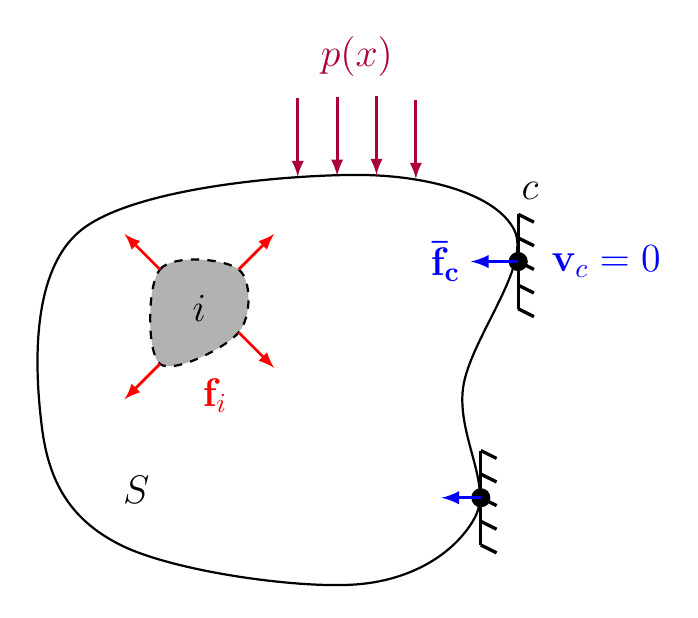
\begin{tikzpicture}[]
 \draw [thick]  plot[smooth cycle, tension=.6] coordinates {(0,2) (0.5,4.5) (4,5.2) (6,4.5)  (5.35,2.5) (5.5,0.85) (4,0) (1,0.5) };
\node[outer sep=0pt,thick] at (1.2,1.2) [] {\Large${S}$};
 
\draw [thick,dashed, fill=white!70!black]  plot[smooth cycle,  tension=.6] coordinates {(1.5,2.8) (1.5,4) (2.5,4)  (2.5,3.2) };

\node[outer sep=0pt,thick] at (2,3.5) [minimum width=1.5cm, minimum height=1.5cm] {\Large$i$};
 
\draw [line width=1pt,red,-latex]  plot[smooth, tension=.6] coordinates { (1.5,2.8) ($(1.5,2.8)+(-0.45,-0.45)$) }; 
\draw [line width=1pt,red,-latex]  plot[smooth, tension=.6] coordinates { (1.5,4) ($(1.5,4)+(-0.45,0.45)$) }; 
\draw [line width=1pt,red,-latex]  plot[smooth, tension=.6] coordinates { (2.5,4) ($(2.5,4)+(0.45,0.45)$) }; 
\draw [line width=1pt,red,-latex]  plot[smooth, tension=.6] coordinates { (2.5,3.2) ($(2.5,3.2)+(0.45,-0.45)$) }; 

\node[outer sep=0pt,thick] at (2.2,2.4) [] {{\color{red}\Large$\mathbf{{f}}_{i}$}};

\node[outer sep=0pt,thick] at ($(3.25,5.2)+(0.75,1.5)$) [] {{\Large\color{black!10!purple}$ p(x)$}};

 \draw [line width=1pt,color = black!10!purple,latex-]  plot[smooth, tension=.6] coordinates { (3.25,5.175) ($(3.25,5.175)+(0,1)$) }; 
  \draw [line width=1pt,color = black!10!purple,latex-]  plot[smooth, tension=.6] coordinates { ($(3.25,5.19)+(0.5,0)$) ($(3.25,5.19)+(0.5,1)$) }; 
  \draw [line width=1pt,color = black!10!purple,latex-]  plot[smooth, tension=.6] coordinates { ($(3.25,5.2)+(1,0)$) ($(3.25,5.2)+(1,1)$) }; 
    \draw [line width=1pt,color = black!10!purple,latex-]  plot[smooth, tension=.6] coordinates { ($(3.25,5.15)+(1.5,0)$) ($(3.25,5.15)+(1.5,1)$) }; 


% \begin{scope}[xshift=6.25cm,yshift=4.8cm, rotate=-15.5]
% \draw [thick]  plot[smooth cycle, tension=.6] coordinates {(0,-1) (1,-4.5) (6,-4.5) (5,-1) (1,0.3) };
% \node[outer sep=0pt,thick] at (5.5,-4) [] {\Large${R}$};
 
% \draw [line width=3pt,black,cap=round]  plot[smooth, tension=.6] coordinates {  (6,-4.5) (5.2,-4.8) (4.5,-4.9) };  
% \node[outer sep=0pt,thick] at (5.5,-5.2) [] {\Large$b$};

% \end{scope}

\draw[very thick, black, fill=black] (6.05,4.1) circle[radius=.1];

\draw[very thick, black] (6.05,3.5) -- (6.05,4.7);
\draw[very thick, black] (6.05,3.5) -- ($ (6.05,3.5) + (0.2,-0.1) $);
\draw[very thick, black] (6.05,4.7) -- ($ (6.05,4.7) + (0.2,-0.1) $);
\draw[very thick, black] (6.05,4.1) -- ($ (6.05,4.1) + (0.2,-0.1) $);
\draw[very thick, black] (6.05,4.4) -- ($ (6.05,4.4) + (0.2,-0.1) $);
\draw[very thick, black] (6.05,3.8) -- ($ (6.05,3.8) + (0.2,-0.1) $);
\draw[very thick, blue,-latex] (6.05,4.1) -- (5.45,4.1) node[left,pos=1] {\Large$\color{blue}\mathbf{\bar{f}_c}$};


\draw[very thick, black, fill=black] (5.575,1.1) circle[radius=.1];
\draw[very thick, black] (5.575,0.5) -- (5.575,1.7);
\draw[very thick, black] (5.575,0.5) -- ($ (5.575,0.5) + (0.2,-0.1) $);
\draw[very thick, black] (5.575,1.7) -- ($ (5.575,1.7) + (0.2,-0.1) $);
\draw[very thick, black] (5.575,1.1) -- ($ (5.575,1.1) + (0.2,-0.1) $);
\draw[very thick, black] (5.575,1.4) -- ($ (5.575,1.4) + (0.2,-0.1) $);
\draw[very thick, black] (5.575,0.8) -- ($ (5.575,0.8) + (0.2,-0.1) $);
\draw[very thick, blue,-latex] (5.575,1.1) -- (5.075,1.1) node[left,pos=1] {};

\node[right] at (6.35,4.1) {\Large $\color{blue}\mathbf{v}_c = 0$};

\node[outer sep=0pt,thick] at (6.2,5) [] {\Large$c$};
  
 \end{tikzpicture}
\end{document}